% (This file is included by thesis.tex; you do not latex it by itself.)

\begin{abstract}

% \begin{center}
%     \textit{``An ancient time\\
%     When compass needles lost their way; \\
%     Finding North from South." \\}
%     \vspace{10pt}
%     S. W. Bogue
% \end{center}
Magnetism has had a pivotal role in human history. The first descriptions of magnetic stones (i.e. lodestones) in ancient China date back to before 200 BC. By the eleventh century, compasses made of magnetic needles had been widely used for navigation purposes in China. Through the Silk Road, Chinese compass made its way to Europe and became an essential tool for navigation during the Age of Discovery. Advances in our understanding of electromagnetism since the second Industrial Revolution facilitated the rapid increase in the inter-connectivity of cultures around the globe. Today's civilization is very much dependent on the electricity generated by the giant rotating magnets in power plants. 

A compass can help navigate is because the magnetic minerals in the compass needle tend to align with Earth's dominantly dipolar magnetic field. In the rock records, there are numerous microscopic compasses that are carrying ancient magnetic records through deep time. These microscopic compasses are magnetic minerals such as iron-titanium oxides that occur rather ubiquitously in igneous, sedimentary, and metamorphic rocks. Being rooted in understanding of rock formation processes and the physics of electromagnetism, the study of paleomagnetism utilizes these magnetic compasses in rocks to explore Earth history topics.

In this dissertation, I find my applications of paleomagnetism in reconstructing late Proterozoic magmatism, geomagnetic field behavior, and paleogeography. In chapter 1, I develop paleomagnetic directional data and pair them with geochemical, geochronological, and petrographic data to study the characteristics of mafic magmatism associated with the emplacement of the 1.1 billion-year-old anorthosite xenolith-bearing Beaver River diabase and the extrusive Greenstone lava flow. In chapter 2, I develop paleointensity data from anorthosite xenoliths of the Beaver River diabase to gain insight into the strength of the geodynamo at the time. In chapter 3, I develop paleomagnetic directional data from the Neoproterozoic Jacobsville Formation to constrain global paleogeography during the assembly of the supercontinent Rodinia. In chapter 4, I develop paleomagnetic directional data from 1.1 billion-year-old mafic intrusions and lava flows in the Death Valley and the Grand Canyon to interrogate the extent of the southwestern Laurentia large igneous province and its temporal-magmatic relationship with the Midcontinent Rift. 

\subsection{Late Mesoproterozoic magmatism in the Midcontinent Rift and the southwestern Laurentia large igneous province}

The ancient North American craton, Laurentia, first formed in the Paleoproterozoic Era when a series of collisional orogenies culminating the Trans-Hudson orogeny led to the amalgamation of Archean provinces \citep{Hoffman1988a, Whitmeyer2007a}. The craton continued to grow through the rest of the Paleoproterozoic and into the Mesoproterozoic via accretionary orogenesis along its margin. In the latest Mesoproterozoic (ca. 1110 to 1080 Ma), the large intracontinental Midcontinent Rift (Fig. \ref{fig:abstract_overview}), which was co-located with a large igneous province (LIP) \citep{Swanson-Hysell2021a} led to extension within the Archean Superior province and adjacent Paleoproterozoic provinces to the south \citep{Cannon1992a}. Magmatic activities punctuated by rapid and voluminous emplacement of extrusive and intrusive rocks in the rift led to the emplacement of a thick succession of volcanic rocks and associated mafic intrusions in Laurentia’s interior. Syn- to post-rift thermal subsidence led to deposition of clastic sedimentary rocks on top of the igneous rocks.

\begin{figure}[h!]
    \centering
    \includegraphics[width=0.9\textwidth]{figure/chapters_overview.pdf}
    \caption[Overview of thesis study area and geochronology data]{(A) Simplified map of North America showing the extent of the 1.1 Ga Midcontinent Rift (purple) and the inferred extent of the southwestern Laurentia large igneous province (SWLLIP) based on available high-precision geochronology data. The inset boxes show the areas of study of the dissertation chapters. (B) Compilation of chemical abrasion-isotope dilution-thermal ionization mass spectrometry (CA-ID-TIMS) zircon U-Pb geochronology data from the Midcontinent Rift and southwestern Laurentia. Data are from \citep{Fairchild2017a, Swanson-Hysell2014a, Swanson-Hysell2019a, Mohr2024a}. The colored zones represent the estimated duration of the pulsed and voluminous magmatic events in Laurentia ca. 1.1 Ga.}
    \label{fig:abstract_overview}
\end{figure}

The Midcontinent Rift eventually failed to split the continent into two. Far-field compressional forces associated with the onset and development of the Grenvillian orogeny along the eastern margin of Laurentia led to cessation and subsequent inversion of the rift \citep{Cannon1993a, Swanson-Hysell2019a}. In the southern Lake Superior region, Midcontinent Rift volcanic and sedimentary rocks were uplifted along with Paleoproterozoic and Archean lithologies via thrust faults, forming the crustal-scale Montreal River monocline \citep{Cannon1993a}. The resultant topography led to erosion and the deposition of the early Neoproterozoic Jacobsville Formation \citep{Hamblin1958a, Kalliokoski1982a, Hodgin2022a}, which overlies an angular unconformity that developed on lithologies that were exhumed through this earlier episode of contractional deformation associated with Grenvillian orogenesis. 

The intracontinental nature of the rift and its cessation led to a large amount of rift rocks being preserved in the interior of Laurentia far from continental margins. Rocks in the rift subsequently experienced mild burial and metamorphism history. Rb-Sr dates from the uplifted basement rocks in southern Lake Superior region show that the area has not been heated to above $\sim$300 \textdegree C since ca. 1050 Ma \citep{Cannon1993a}. $^{10}$Be data show that some surface bedrock exposures have only recently been near the surface due to Pleistocene glacial and recent fluvial erosion \cite[e.g.][]{Ullman2015a}. 

The well-preserved Midcontinent Rift rocks provide a wealth of opportunities for characterizing the magmatic history of Laurentia at the time. Geochronology and geochemistry data have been used to group magmatic activities in the rift into four stages based on interpreted changes in relative magmatic volume and the nature of magmatism: early ($\sim$1109--1104 Ma), latent ($\sim$1104--1098 Ma), main ($\sim$1098--1090 Ma) and late ($\sim$1090--1083 Ma) \citep{Vervoort2007a, Heaman2007a, Miller2013a}. In recent decades, the development of the chemical abrasion-isotope dilution-thermal ionization mass spectroscopy (CA-ID-TIMS) enabled high-precision measurement of zircon U-Pb ages in the deep time. In the Midcontinent Rift, these data have been combined with the high-quality paleomagnetic data from the extrusive and intrusive rocks. The data show that Laurentia experienced rapid plate tectonic motion with a speed that reached up to $\sim$30 cm/yr during the development of the Midcontinent Rift \citep{Swanson-Hysell2019a, Rose2022a}. These data also show that distinct rapid and voluminous episodes of magmatism in the rift during the overall protracted period of magmatic activities that lasted $\sim$25 Myr \citep{Swanson-Hysell2019a, Swanson-Hysell2021a, Zhang2021b}. In particular, a large igneous province, consisting of the massive mafic intrusions of the Duluth Complex and associated $\sim$8 km thick extrusive lava flows of the North Shore Volcanic Group, formed within 500 Kyr ca. 1096 Ma \citep{Swanson-Hysell2021a}. Stratigraphically above the Duluth Complex, the ca. 1092 Ma mafic Beaver Bay Complex represents another rapid and voluminous pulse of magmatism. It features the emplacement of the hypabyssal intrusions of the Beaver River diabase that has wide magma conduits containing large anorthosite xenoliths that can be as much as 300 meters wide. Unlike the Duluth Complex and the North Shore Volcanic Group, whose magmatic linkage is supported by the exposed stratigraphic relationships and geochronologic data, there is no direct exposure of volcanic rocks that overlie conformably on top of the Beaver River diabase. Previously, on the basis of geochemical data and petrographic observations, a hypothesis was put forward that the Greenstone Flow of the Portage Lake Volcanics that outcrop in the upper Keweenaw Peninsula in Michigan could be the surface expression of the Beaver River diabase \citep{Doyle2016a}. In chapter 1, I test this hypothesis by using paleomagnetic and geochronologic data to investigate the synchroneity of the emplacement of the intrusive and extrusive rocks (Fig. \ref{fig:abstract_overview}). The data support that the Beaver River diabase was the feeder system for the $\sim$400 meters thick Greenstone Flow which ranks one of the largest lava flows known on Earth. In chapter 2, I utilize the exceptionally well-preserved anorthosite xenoliths hosted in the Beaver River diabase to shed new light on the strength of Earth's geodynamo in the late Mesoproterozoic.

While rapid and voluminous mafic magmatism occurred in the Midcontinent Rift, CA-ID-TIMS zircon U-Pb geochronologic data and paleomagnetic data show that distinct episodes of mafic magmatism occurred in southwestern Laurentia ca. 1098 Ma and ca. 1082 Ma (Fig. \ref{fig:abstract_overview}; \citealp{Mohr2024a}). During a period of $<$0.25 Myr ca. 1098 Ma, thick mafic diabase sills and dikes intruded into the crystalline basement rocks and Mesoproterozoic sedimentary rocks in southwestern Laurentia. The Mesoproterozoic sedimentary successions that contain these intrusions include the Crystal Spring Formation in the Death Valley, Unkar Group sedimentary rocks in the Grand Canyon, and the Apache Group sedimentary rocks in central Arizona \citep{Bright2014a}. The tempo and extent of this episode of mafic magmatism\citep{Mohr2024a}, together with their juvenile geochemical signatures \citep{Hammond1990a, Bright2014a} are interpreted to be consistent with them being driven by an upwelling mantle plume. That the emplacement of the voluminous intrusions in the southwest occurred 2 Myr prior to the Duluth Complex led \citep{Mohr2024a} to invoke a model where the mantle plume first arrived ca. 1098 Ma in southwestern Laurentia and laterally transported toward the readily thinned crust of the Midcontinent Rift. That study posits that the arrival of the plume material in the rift postdates the latent magmatic stage ($\sim$1104--1098 Ma) and led to a replenishment of mafic magma and heat supply in the rift, which eventually drove the emplacement of the ca. 1096 Ma Duluth Complex and the associated lava flows of the North Shore Volcanic Group. In chapter 3, I update the extent of the southwestern Laurentia large igneous province by developing new paleomagnetic data that are paired with new high-precision geochronology data from \cite{Mohr2024a} and by developing additional paleomagnetic data from undated mafic units. 

As the continent-scale Grenvillian orogeny commenced along Laurentia's eastern margin \citep{Swanson-Hysell2019a}, its plate speed slowed down and magmatism in Laurentia waned. The orogenesis also led to the assembly of the supercontinent Rodinia \citep{Swanson-Hysell2023a}. However, there is lack of well-dated paleomagnetic data from Laurentia for constraining global paleogeography between the end of the Mesoproterozoic and the late Tonian (ca. 1050 Ma and ca. 775 Ma; \citealp{Swanson-Hysell2023a, Eyster2019a}). With new geochronologic data that constrain the depositional age of the Jacobsville Formation to be ca. 990 Ma \citep{Hodgin2022a}, in chapter 4 I develop new paleomagnetic data from the Jacobsville Formation in a detailed stratigraphic context and provide a first robust anchor for global paleogeography in the earliest Neoproterozoic. 

\subsection*{The GAD hypothesis in the late Mesoproterozoic}

Earth's magnetic field today is dominated by the dipole component \citep{Alken2021a}. It is the working hypothesis that the time-averaged Earth's surface magnetic field approximates a geocentric axial dipole (GAD)---one produced by a single magnetic dipole at the center of the Earth and aligned with the rotation axis that grants power to paleomagnetic interpretations (Fig. \ref{fig:GAD}). In the GAD model, an observation of an inclination of magnetization ($I$) uniquely corresponds to a latitude value ($\lambda$) (Fig. \ref{fig:GAD}). This relationship is expressed in the ``dipole equation" 
\begin{equation*}
    tan(I) = 2 tan(\lambda)
\label{direction_eq}
\end{equation*} 

The GAD hypothesis also empowers paleomagnetic field intensity observations in that there is a unique correlation between an observed field strength at a latitude and the axial dipole moment (Fig. \ref{fig:GAD}), which is expressed as 
\begin{equation*}
    H = \frac{M\sqrt{1+3cos^2\theta}}{r^3}
\label{intensity_eq}
\end{equation*} Where H is the observed magnetic field intensity, M is the magnetic moment of Earth, $\theta$ is colatitude where $\theta=90-\lambda$, and r is Earth's radius. 

% add inclination-latitude figure and geomagnetic field-dipole moment strength paired plot
\begin{figure}[h!]
    \centering
    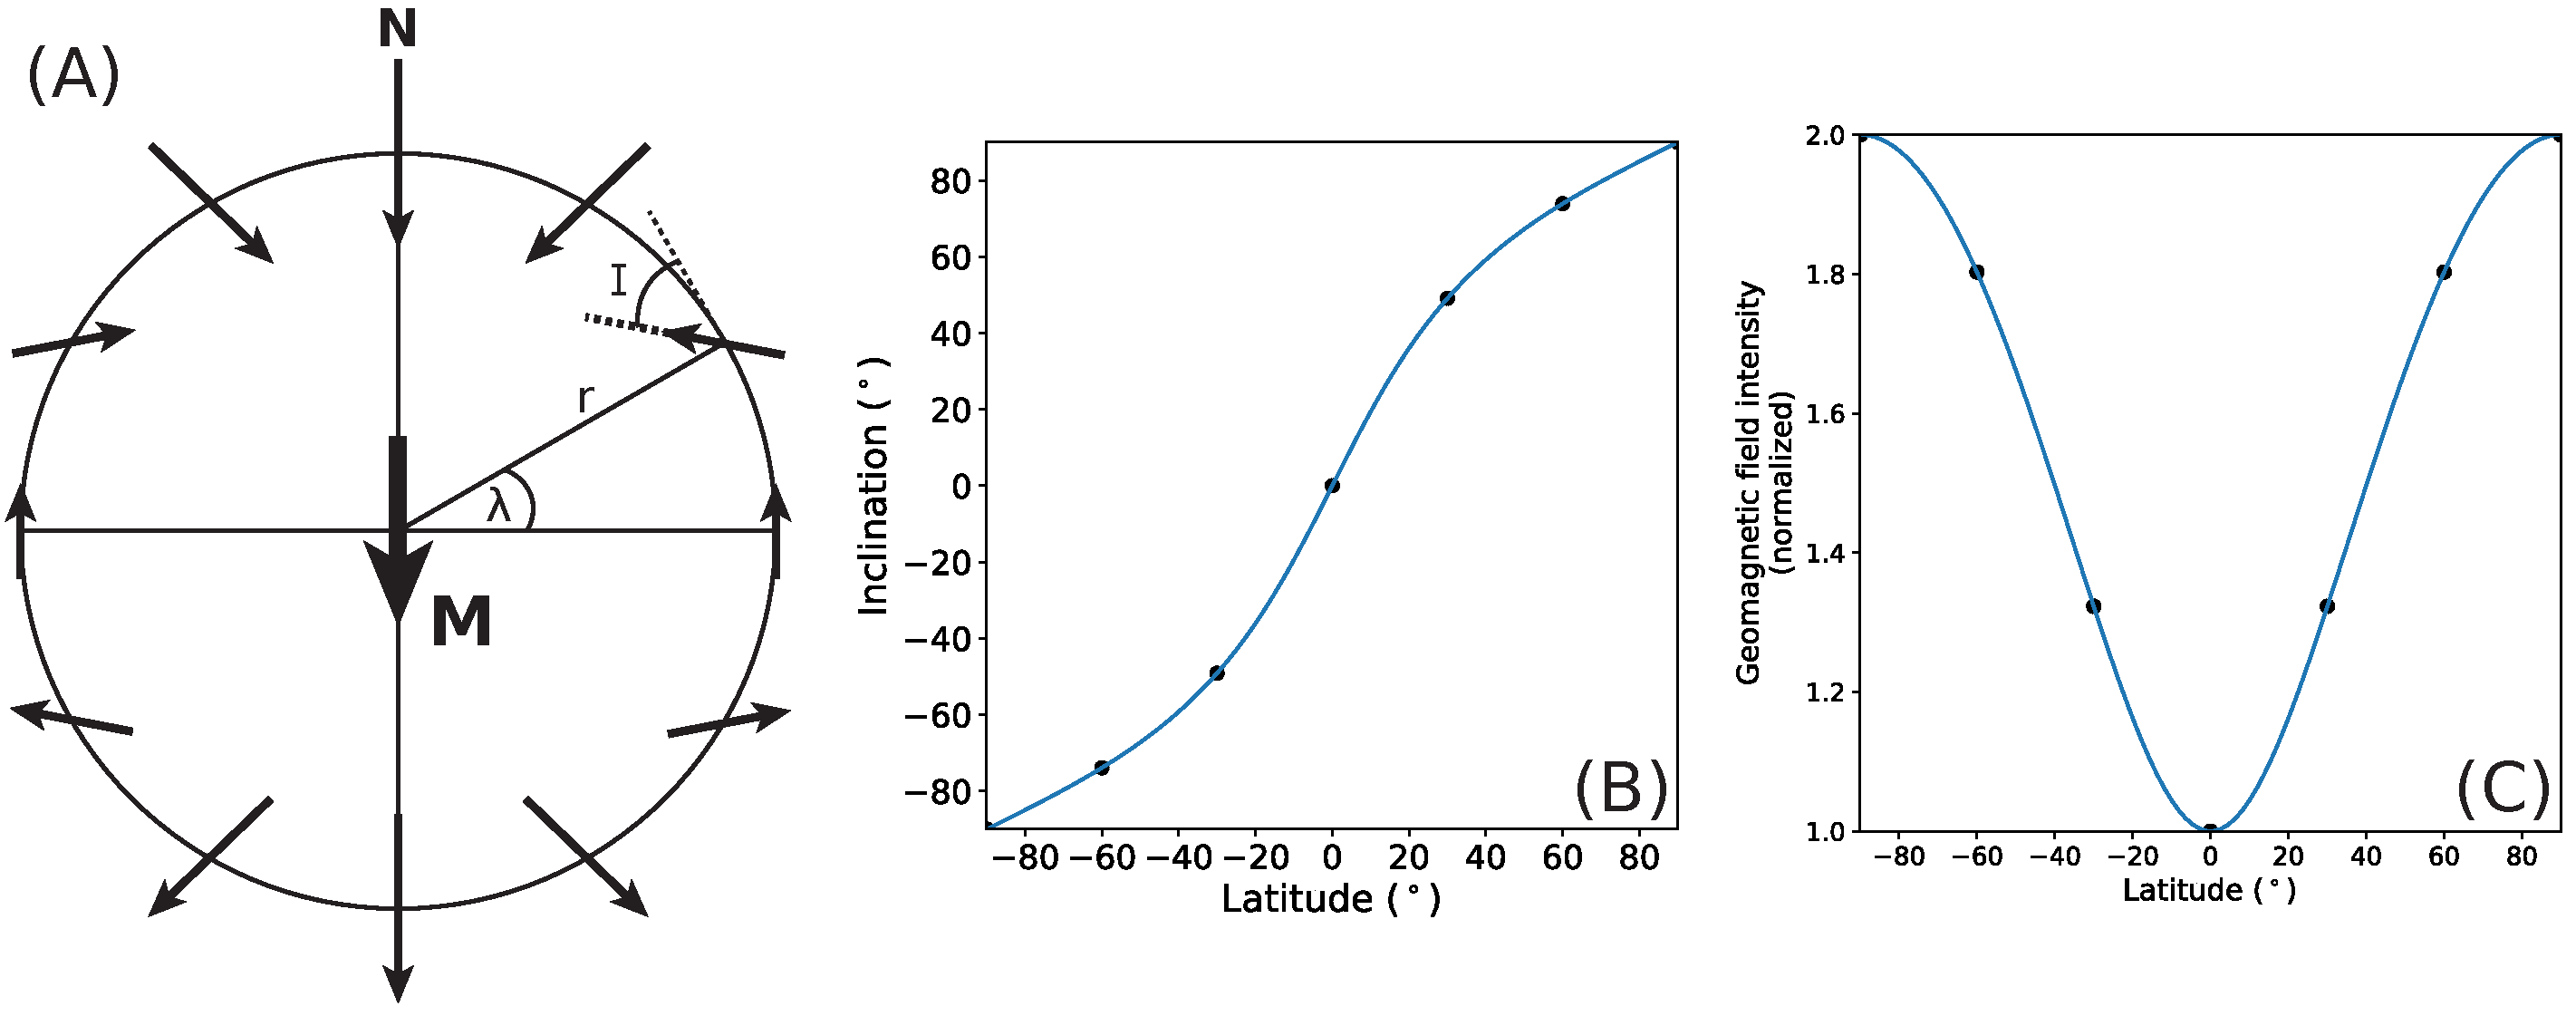
\includegraphics[width=\textwidth]{figure/GAD.pdf}
    \caption[The GAD hypothesis]{(A) Geocentric axial dipole model. Magnetic dipole M is placed at the center of the Earth and aligned with the spin axis; the geographic latitude is $\lambda$; the mean Earth radius is $r$; the magnetic field directions and relative intensities at Earth’s surface produced by the geocentric axial dipole are schematically shown by the arrows; inclination, $I$, is shown for one location; N is the geographic north pole. Modified after \cite{McElhinny1973a}. (B) Correlation between magnetic field inclination and latitude of a dipolar magnetic field. (C) Correlation between latitude and normalized magnetic field intensity produced by a dipolar magnetic field. The intensities are normalized by the field at the equator. }
    \label{fig:GAD}
\end{figure}

Effective ways of testing the robustness of the GAD hypothesis through time include comparing observed latitudinal dependence of paleomagnetic inclination data and intensity data with those predicted by the dipole equations. In addition, the symmetry of paleomagnetic reversals also provides insights into the dipolarity of the field. A geomagnetic field with a dominant non-dipolar component that does not reverse and a reversing dipolar component with minor contributions would have asymmetric reversals. It has been demonstrated that the GAD hypothesis is robust for the past 10,000 years on the basis of global compilations of archeological sites and sediments \cite[e.g.][]{McElhinny1996a}. For the past 5 million years, compilations of paleomagnetic data are best described with a GAD-dominated field with minor persistent contributions from non-dipole components (1-5 \%; \citealp{Tauxe2005a, Valet2011b}). Statistical analyses of compilations of the relatively abundant paleomagnetic directional and intensity data further back in time show that Earth's magnetic field has been compatible with being GAD-dominated throughout the Phanerozoic \citep{Evans1976a, Lhuillier2023a}. The use of paleomagnetic data under the GAD assumption lies at the core of reconstructing past plate tectonic configurations \citep{Creer1954a, Irving1977a, Besse2002a, Torsvik2012a}. The GAD model gains support in the Phanerozoic in that the reconstructed plate motions are smooth with rates typically $<$20 cm/y \citep{Torsvik2012a}. Such results are independently verified by marine magnetic anomalies and hotspot tracks since the mid-Mesozoic \citep{Doubrovine2012a, Muller1993a}.

However, some Precambrian paleomagnetic observations challenge the uniformitariansm of a dipolar geomagnetic field through deeper time. There is increasing evidence that suggest Earth's magnetic field in the Ediacaran may not be GAD-dominated. Anomalously rapid changes in paleomagnetic field directions have been found in rocks from a variety of localities \cite[e.g.][]{Abrajevitch2010a, Meert2014a, Halls2015a}. Magnetostratigraphy data developed by \citep{Kodama2021a} show the Ediacaran Johnnie Formation records anomalously frequent reversals ($\sim$13 per Myr). A series of low paleointensity values have been obtained primarily using single silicate crystals (i.e. dominantly monomineralic crystal aggregates) from Ediacaran rocks \citep{Bono2019a, Thallner2021a, Thallner2021b}. All these data have led some literature to invoke a hypothesis that Earth's magnetic field was not GAD-dominated in the Ediacaran Period. Some have posited that the very low paleointensity observations in the Ediacaran indicate a time when the strength of the geodynamo reached its minimum prior to a recovery brought by the onset of inner core nucleation \cite[e.g.][]{Bono2019a}. Today, the characteristics of the geodynamo in the Ediacaran remain enigmatic, and the mechanism for the anomalous directional and intensity data remains debated \citep{Domeier2023a}.

In the Proterozoic, it had also been previously hypothesized that non-dipole components dominated the geomagnetic field. Prior to the development of high-precision geochronology data that are paired with detailed paleomagnetic data within a volcanostratigraphic context in the Midcontinent Rift became available, the apparent asymmetry in paleomagnetic field reversal records in the Midcontinent Rift rocks led the literature \citep[e.g.][]{Halls1982a, Pesonen1981a} to interpret there being a significant non-GAD field component in the late Mesoproterozoic. However, high-resolution paleomagnetic data that span three geomagnetic field reversals in a stratigraphic context show each reversal was symmetric \citep{Swanson-Hysell2009a}. Since that work, more data and sophisticated statistical analyses have further clarified that the paleomagnetic pole progression recorded by rocks of the Midcontinent Rift most likely represent a period of rapid plate tectonic motion of Laurentia. Nonuniformitarian events such as there being significant non-GAD geomagnetic field components or a significant and long-lasting true polar wander event need not be invoked 
in the late Mesoproterozoic \citep{Swanson-Hysell2019a, Rose2022a}. 

Additional statistical analyses also show that the Proterozoic geomagnetic field is consistent with being dipole-dominated. \cite{Tauxe2009a} show that the shape of the distribution of the paleomagnetic directional data recorded by lava flows of the North Shore Volcanic Group in the Midcontinent Rift is consistent with that of the past 5 million years (model TK03 of \cite{Tauxe2004b}). My collaborative work with \citep{Pierce2022a} also show that correcting the inclination shallowing of syn-rift hematite-bearing sedimentary rocks of the Cut Face Creek Sandstone based on the geomagnetic field model of TK03 results in a mean direction that agrees with that recorded by the volcanic rocks that bracket the sedimentary rocks. These analyses support the interpretation that the geomagnetic field at Midcontinent Rift time was consistent with being dipole-dominated and had a secular variation pattern similar to that of recent geologic times. In addition, the analyses of \citep{Gong2023a} show that the available paleomagnetic directional observations across Laurentia in the Proterozoic can be better fit with a dipole than a quadrupole configuration. Overall, the enriching paleomagnetic directional and intensity data in the Proterozoic have been adding increasing support for there being a GAD-dominated geomagnetic field through the Proterozoic Eon \citep{Veikkolainen2014a, Salminen2017a, Veikkolainen2021a}. 

With confidence in the GAD-dominated field in the Mesoproterozoic, we can utilize paleomagnetic directional data to explore temporal associations between rock units. In chapter 1 I develop new paleomagnetic data from the ca. 1092 Ma Beaver River diabase and compare their pole position to that of the Greenstone Flow of the Portage Lake Volcanics. The agreement between the pole positions between the extrusive and intrusive rocks indicate a close temporal linkage and support a magmatic linkage between the two units. In chapter 3, I develop new paleomagnetic data from mafic intrusive and extrusive rocks in southwestern Laurentia and investigate the extent of the southwestern large igneous province, and its temporal and magmatic relationship with the Duluth Complex. These new data add to the existing paleomagnetic database for Laurentia for the reconstruction of the Keweenawan Track---the the late Mesoproterozoic apparent polar wander path of Laurentia which is central to the reconstruction of global paleogeography leading up to the assembly of the Rodinia supercontinent. 

\subsection{Probing the evolution of Earth's interior via paleointensity observations}

Earth's magnetic field is powered by convective flow of liquid iron-alloy in Earth's outer core. At present day, the geodynamo is collectively driven by heat flow across the core-mantle boundary and from the crystallization of the solid inner core from the liquid outer core which provides latent heat and compositional buoyancy due to the exclusion of light elements \citep{Buffett2000a}. The global entropy balance for the convective core that relates the Ohmic dissipation to thermal and compositional convection show that the compositional convection is more efficient in maintaining the current energy dissipation \citep{Labrosse2003a, Landeau2022a}. A question thus arise regarding whether Earth has had an inner core since the beginning of its formation, and if not, when did the inner core begin to nucleate. Theoretical calculations show large uncertainties associated with the predicted timing of the inner core nucleation \citep[e.g.][]{Buffett2003a, Pozzo2012a, Nimmo2015a} due to the lack of constraints on the thermal conductivity of the core \citep{Gubbins2004a, Konopkova2016a, Ohta2016a}. Such uncertainties remain until further constraints on the core composition and agreements on experimental results of thermal conductivity values of iron-alloy at Earth's core conditions become available in the literature. 

Paleomagnetic observations provide a unique tool that can provide constraints on the thermal evolution of Earth’s core. Based on paleomagnetic directional and intensity data, we know that an active dynamo has existed since the 3.5 Ga \citep{Selkin2007a, Biggin2011a, Tarduno2014a, Brenner2020a, Brenner2022a} and probably earlier \citep{Tarduno2015a}. Theory and modeling predict that the nucleation of the inner core would produce a notable increase in the efficiency of convection in the outer core such that a notable increase in the surface geomagnetic field intensity may be observed and thus be reflected in the paleomagnetic intensity records \cite[e.g.][]{Labrosse2003a, Aubert2009a, Driscoll2016a, Landeau2022a}. 

Paleointensity experiments are used to reconstruct records of past absolute geomagnetic field intensity from thermoremanent magnetizations based on the linear dependence of thermal remanence acquisition on the magnetic field present. Based on the single domain thermal remanence magnetization blocking theory of \cite{Neel1955a}, \cite{Butler1992a} deduced the following equation for the acquisition of thermal remanence magnetization (TRM) of a population of identical single-domain ferromagnetic grains when cooling in a constant magnetic field (H) from the blocking temperature ($T_B$) to ambient temperature ($T_0$):
\begin{equation*}
    TRM [T_0] = N[T_B] v j_s [T_0] tanh(\frac{v j_s [T_B]H}{k T_B})
\label{PINT_eq_1}
\end{equation*}
where $[T_0], [T_B]$ denote the temperature of the temperature-dependent parameters, $N[T_B]$ represents the number of single-domain grains per unit volume with blocking temperature $T_B$, $v$ is the volume of the single domain grains and $j_s$ is the saturation magnetization, k is the Boltzmann constant. This equation assumes the grains block in the remanence magnetization sharply when cooling through the blocking temperature $T_B$. Typically the term $\frac{v j_s [T_B]H}{k T_B}$ which measures the degree of alignment of the grains at the blocking temperature has a value $<<1$. Therefore, equation \ref{PINT_eq_1} becomes 
\begin{equation*}
    TRM [T_0] = AH
\label{PINT_eq_2}
\end{equation*}

where A is a generalized proportionality constant. A rock sample that acquires a thermal remanent magnetization that follows this linear relationship with the magnetic field that it cools in would thus have a proportionality constant $A$ which depicts both $TRM_{paleo}=AH_{paleo}$ and $TRM_{lab}=AH_{lab}$, where $H_{paleo}$ represents the ancient field and $H_{lab}$ represents the lab field. Therefore, the paleointensity can be obtained by eliminating the proportionality constant, A, and 
\begin{equation*}
    H_{paleo} = \frac{TRM_{paleo}}{TRM_{lab}}
\label{PINT_eq_3}
\end{equation*}

% add paleointensity example plot
\begin{figure}[h!]
    \centering
    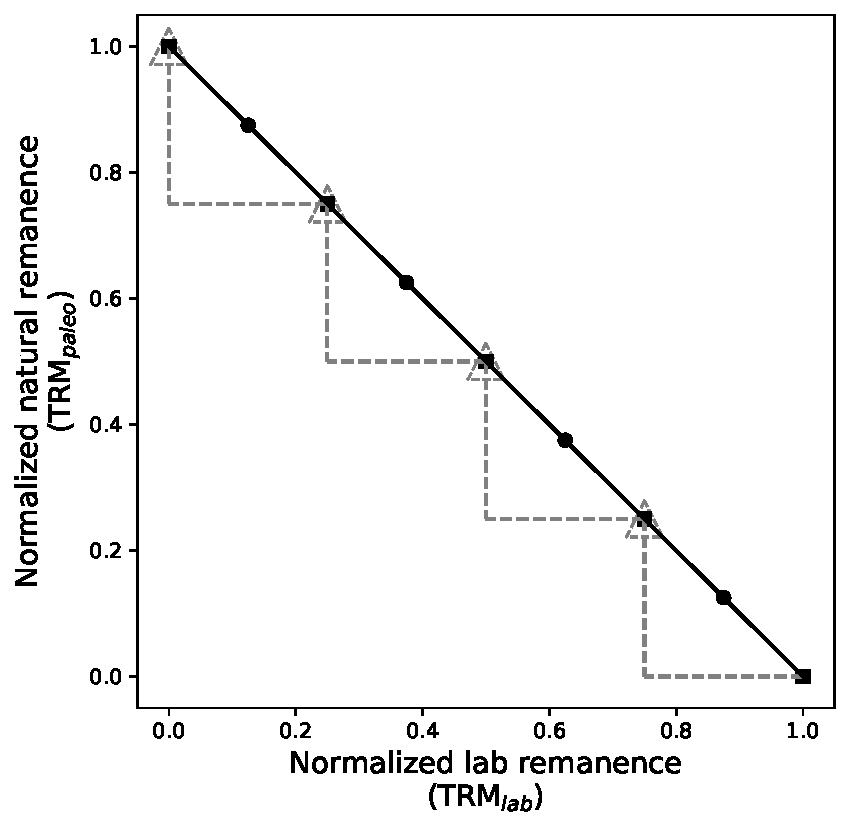
\includegraphics[width=0.6\textwidth]{figure/IZZI_protocol.pdf}
    \caption[Schematic illustration of the IZZI paleointenstiy protocol]{Schematic Thellier paleointensity diagram showing an ideal experimental results using the ``in field-zero field-zero field-in field" paleointensity protocol developed by \citet{Yu2004a}. The squares and circles represent in field or zero field steps. Grey dashed lines and triangles illustrate the pTRM check steps where a repeat TRM acquisition step is performed to test for changes in a specimen's ability to acquire TRM at blocking temperatures below the temperature of the check. }
    \label{fig:IZZI_protocol}
\end{figure}

With this theoretical basis, \cite{Thellier1959a} developed the experimental protocol known as the Thellier double-heating paleointensity method that features step-wise removal of the natural thermal remanence magnetization ($TRM_{paleo}$) and imposition of new partial thermal remanence ($TRM_{lab}$) in a known lab field through heating and cooling. This technique is based upon Thellier’s laws, which state that partial thermal remanence (pTRM) must be additive, independent (partial remanence acquired between distinct temperature steps is distinct from one another) and reciprocal (the unblocking temperature is the same as the blocking temperature. The resultant comparison between a sample's capability of acquiring a TRM in the lab and its acquired TRM in nature is then illustrated in the paleointensity plot first introduced by \cite{Arai1963a} (Fig. \ref{fig:IZZI_protocol}). In an ideal experiment with ideal magnetic recorders, the relationship between natural remanence lost and pTRM gained is linear, and the slope of the best-fit line to the data is proportional to the intensity of the ancient field (Fig. \ref{fig:IZZI_protocol}. Using this slope, and multiplying by the known lab field, one can calculate the ancient magnetic field strength. The Thellier method has subsequently been improved such that sample behaviors that diverge from being ideal single-domain described in the theory above can be better detected \citep[e.g.][]{Coe1967b, Riisager2001a, Yu2003a, Yu2004a, Yu2006a}. Today, the ``in field-zero field-zero field-in field" (IZZI) Thellier paleointensity protocol combined with result filtering based on a series of statistical selection criteria is one of the most robust and widely used heating-based methods \citep{Yu2004a}. 

With the GAD assumption, Earth's (virtual) axial dipole moment can be calculated given known paleointensity and paleolatitude of a locality at a time. There are compilations of absolute paleointensity data that show Earth's axial dipole moment through history \citep[e.g.][]{Veikkolainen2014b, Bono2022b}. Based on a selected compilation, \citep{Bono2019a} interpreted that the existing Precambrian paleointensity database shows a monotonic decay of the geomagnetic dipole moment throughout the Proterozoic. Together with their new data developed from silicate crystals of the ca. 565 Ma Sept-$\hat{I}$les mafic intrusions with the Thellier–Coe paleointensity method which were interpreted to show near-zero values, \cite{Bono2019a} hypothesized that a geodynamo primarily driven by waning thermal convection might have persisted through the Proterozoic until the nucleation of the inner core, which they interpreted to have happened in the Ediacaran. \cite{Bono2019a} further argued that their results are consistent with modeling results using an approach combining dynamo simulations and theoretical scaling relationships that predicted that progressive decay of the field’s dipole moment would be followed by a rapid increase in geomagnetic field intensity soon after the onset of inner core nucleation such that a minimum in dipole moment would occur just before inner core nucleation \citep{Driscoll2016a}. 

However, the geodynamo evolution model put forward by \citep{Bono2019a} was based on a sparse Precambrian paleointensity database and is challenged by more recent observations. Low paleointensity values similar to those in the Ediacaran have been observed in the Mesoproterozoic \citep{Lloyd2021b, Shcherbakova2022a, Shcherbakova2023a}, the Neoproterozoic \citep{Lloyd2021a}, the early-Cambrian \citep{Lloyd2022a}, and the Paleozoic \citep{Shcherbakova2021a}. These new data challenge the uniqueness of the Ediacaran weak geodynamo. In chapter 2, I develop new paleointensity data from the ca. 1092 Ma anorthosite xenoliths of the Beaver River diabase. The paleomagnetic directional data I developed in chapter 1 establish that the anorthosite xenoliths are stable remanence recorders that acquired remanence during cooling in the host diabase. I then used the ``IZZI" Thellier paleointensity protocol \citep{Yu2004a} to develop absolute paleointensity data from the same xenoliths and calculated the axial dipole moment of Earth's magnetic field. My data together with previous observations from rocks of the Midcontinent Rift show high paleointensity values ca. 1.1 Ga. Some of the xenoliths unequivocally show exceptionally high paleointensity values. Those high values require there being a strong dynamo in the late Mesoproterozoic, which does not fit in the interpreted Proterozoic monotonic decay trend hypothesized by \cite{Bono2019a}. 

Overall, the high paleointensity values of the Beaver River anorthosite xenoliths necessitate a strong late Mesoproterozoic geodynamo. The enriching paleomagnetic database for the Precambrian is revealing a more complex history if Earth's core than previously thought. The observational data from paleomagnetism are now stirring renewed interests in better understanding the core's material properties in deep-Earth conditions and in understanding the dynamic connections between the mantle and the core. 

\subsection{Recovering deep-time paleointensity records from silicate-hosted Fe-oxides}

Successful recovery of deep-time paleomagnetic records is dependent on rocks maintaining primary magnetic remanence through time and having stable behaviors during paleointensity experiments. Rocks are assemblages of fine-grained ferromagnetic particles with various stability that are dispersed within a matrix of diamagnetic and paramagnetic minerals. Not all ferromagnetic particles can maintain a magnetic memory through deep time. The characteristic time through which a ferromagnetic grain is capable of maintaining a magnetization before spontaneous relaxation is a function of temperature, external magnetic field, composition, size, and shape \citep{Neel1955a}. Theoretical derivations show that the most stable remanence carriers are single-domain particles with a narrow size range \citep{Butler1975a, Butler1992a}. For example, ensembles of magnetite grains with sizes ranging from a few tens of nanometers to up to one micron, and hematite grains with sizes up to 15 $\mu$m can maintain a stable magnetization for billions of years. Recent advances in micromagnetic modeling and fine-scale magnetic imaging show that stable ferromagnetic particles in geologic samples are likely to be more often in the single vortex state which behaves similarly to the single domain state \citep{Nagy2017a, Tauxe2020a, CortesOrtuno2022a}. 

Other ferromagnetic particles in rocks include multidomain grains (i.e. particles with multiple magnetic domains) and grains with complex vortex states (or pseudo-single-domain grains) which have more complex magnetic behaviors \citep{Williams2010a}. While some of them may be capable of maintaining primary paleomagnetic directional records through deep time, others are more prone to having their magnetizations be overwritten by heating or prolonged immersion in Earth's magnetic field postdating the acquisition of the primary remanence. Results of such processes typically manifest in rock samples as superposition of secondary remanence components on top of variably preserved primary remanence. 

While isolation of primary paleomagnetic directional data from secondary overprints is possible via step-wise thermal demagnetization experiments and vector subtractions, the existence of multidomain and complex vortex state grains complicate the determination of paleointensity records as their remanence acquisition and removal behaviors deviate from the Thellier laws. In addition, alteration of rocks in nature and in the lab can also complicate paleomagnetic records by changing the magnetic mineralogy. This includes destruction of original minerals and formation of new magnetic minerals associated with chemical alteration during heating in the lab. Such mineralogical alterations are detrimental to paleointensity experiments, since the acquired remanence during the in-field steps in the lab would be held by grains distinct from those that record the natural remanence. Due to such complexities, recovering deep time paleointensity records is usually more difficult than recovering paleomagnetic directional records. 

It has been found that ferromagnetic grains enshrouded by silicate mineral hosts can be well-protected from alteration and be faithful paleointensity recorders \citep{Cottrell1999a, Cottrell2000a, Tarduno2005a, Tarduno2005a, Tarduno2006a, Cottrell2008a, Selkin2000a, Selkin2007a, Selkin2008a}. In particular, titanomagnetite grains hosted in plagioclase crystals are intriguing targets. Petrography, electron microscopy, and microprobe data have shown that minor amount ($<$1\% by weight) of iron commonly exist in plagioclase crystals which can be present as fine-scale magnetite needles \citep{Selkin2000a, Feinberg2005a, Feinberg2006a, Wenk2011a, Bian2021a}. Rock magnetic analyses show that many of the rocks have ferromagnetic mineral assemblages dominated by single-domian-like behaviors with stable remanence carrying abilities. In addition, the alteration of the plagioclase does not readily result in the formation of secondary iron oxides in contrast with Fe-silicate minerals such as olivine and pyroxene. 

In chapter 2, I develop new paleointensity data using the anorthosite xenoliths of the Beaver River diabase in the Midcontinent Rift to characterize Earth's magnetic field ca. 1092 Ma. Electron microscopy images show that plagioclase crystals within these anorthosite xenoliths can enclose small pyroxene crystals which have fine-scale exsolved titanomagnetite grains. These observations corresponds to rock magnetic data that a number of the xenoliths typically have a dominant population of stable single-domain-like particles. The failed intracontinental rift nature of the Midcontinent Rift results in the anorthosite xenoliths being distant from subsequent tectonic events along Laurentian margins such that the lithology and magnetization of the anorthosite xenoliths have been minimally altered following initial formation. 

\subsection{Using detrital remanent magnetization in hematite-bearing sedimentary rocks for paleogeographic reconstructions}

Sedimentary rocks are important archives of Earth history. They provide major contributions to global paleogeography reconstructions \cite[e.g.][]{Torsvik2012a, Domeier2012a, Vaes2023a}. While igneous rocks acquire thermal remanent magnetizations during cooling through blocking temperatures of ferromagnetic minerals \citep{Neel1955a}, sedimentary rocks acquire detrital remanence magnetizations as a result of preferential alignment of detrital ferromagnetic particles with the local magnetic field during deposition. In the Midcontinent Rift, clastic sedimentary rocks of the Oronto Group deposited during post-rift thermal subsidence following the bulk of rift magmatic activity provide paleomagnetic poles that extend the Keweenawan Track to ca. 1070 Ma \citep{Henry1977a, Slotznick2023a}. 

However, the accuracy of paleomagnetic directions recorded by the detrital remanent magnetization of sedimentary rocks has long been recognized as problematic due to the issue of inclination shallowing \citep{King1955a, Kodama2012a, Tauxe1984a, Van-Andel1966a}. The rotation of ferromagnetic grains during deposition and compaction can result in the acquisition of a detrital remanence that is biased shallow relative to the local geomagnetic field in which it was acquired (Fig. \ref{fig:DRM_inclination_shallowing}; \citealp{Tauxe2005a}). Such inclination shallowing effect can be described as 
\begin{equation*}
\textup{tan}(I_o) = f\textup{tan}(I_f)
\end{equation*}
where $I_o$ represents the observed inclination of the specimen magnetization and $I_f$ represents the inclination of the field in which the magnetization was acquired. If uncorrected, shallower inclinations obtained from sedimentary rocks can potentially result in erroneously low estimates of paleolatitudes, biasing the interpreted past positions of continents and hindering plate reconstructions.

\begin{figure}[h]
    \centering
    \includegraphics[width=0.9\textwidth]{figure/DRM_inclination_shallowing.png}
    \caption[The inclination shallowing problem in detrital remanence magnetization]{(A) Schematic illustration of detrital remanence magnetization acquisition process. The existence of Earth's magnetic field biases the orientation of the detrital ferromagnetic particles such that they would be preferentially aligned with the local field direction during deposition. The apparently rotated detrital ferromagnetic grains in the deposited sedimentary layers represent inclination shallowing due to rotation of the grains toward the bedding plane. (B) Reflected petrographic image showing detrital Fe-Ti oxides with bright colors in a matrix dominated by quartz and feldspar grains. (C) The relationship between the inclination of the local magnetic field compared to the observed inclination in sedimentary rock records that experienced various degrees of inclination shallowing is shown. A value of 1.0 corresponds to no flattening while a value of 0.0 means the magnetizations are completely flattened. Figure (A) modified after \cite{Tauxe1993a}. Figure (C) modified after \cite{Pierce2022a}.}
    \label{fig:DRM_inclination_shallowing}
\end{figure}

Experimental methods such as magnetic fabric analyses \cite[e.g.][]{Kodama1995a, Bilardello2010a, Bilardello2010c, Bilardello2010b} as well as statistical approaches \cite[e.g.][]{Tauxe2004b} have been developed for correcting inclination shallowing in sedimentary records. However, there had been limited efforts in reporting uncertainties associated with the amount of shallowing, let alone propagating such uncertainties into paleogeographic reconstructions. We developed a new method for quantifying uncertainties associated with inclination shallowing by using a spherical bivariate Kent distribution to represent uncertainties associated with paleomagnetic mean pole position through collaboration with an undergraduate honors thesis project at Berkeley Earth and Planetary Science which is published as \cite{Pierce2022a}. This method has had successful applications in paleogeography reconstructions \citep{Slotznick2023a, Vaes2023a, Zhang2024a}. 

In chapter 4, I develop new paleomagnetic data from the hematite-bearing sedimentary rocks of the Jacobsville Formation which overlies unconformably on top of Midcontinent Rift. \cite{Hodgin2022a} developed geochronology data that constrain the timing of deposition of the Jacobsville Formation to be associated with compressional deformation of the Grenvillian orogenesis ca. 990 Ma. I used a Kent mean statistics to represent the pole position and associated uncertainty. That pole is the first constraint from Laurentia's interior for the global paleogeography in the earliest Neoproterozoic. In that chapter, I show that the data from the Jacobsville Formation together with the Keweenawan Track support a tectonic model where Laurentia traveled rapidly equatorward in the latest Mesoproterozoic and significantly slowed down following the onset of the Grenvillian orogenesis. 

\subsection{The global paleogeography in the earliest Neoproterozoic: progress and future directions}

The evolution of the configuration of ancient continents is foundational to our knowledge of global tectonics, geodynamics, and climate through Earth history. We know that in the late Proterozoic, ancient continents conjoined together to form the supercontinent Rodinia \citep{Swanson-Hysell2021c}. The position of Laurentia is particularly crucial given its central location in the supercontinent. The Keweenawan Track of Laurentia has become a central record for reconstructing the assembly of Rodinia \citep{Evans2021b}. The Keweenawan Track records rapid equatorward motion associated with the closure of the Unimos Ocean basin between Laurentia and conjugate continents leading up to the collisional Grenvillian orogeny that assembled Rodinia (Fig. \ref{fig:abstract_paleogeography}). The Grenvillian orogeny initiated ca. 1090 Ma with granulite-facies metamorphism of the Ottawan Stage of the orogeny occurring ca. 1050 Ma, but with protracted collisional orogenesis continuing through the 1020 to 980 Ma Rigolet Stage \citep{Rivers2008a, Rivers2012b, Swanson-Hysell2023a}. This later stage of the orogeny led to the formation of the Grenville Front, as contractional deformation propagated further into the continent. 

\begin{figure}[h!]
    \centering
    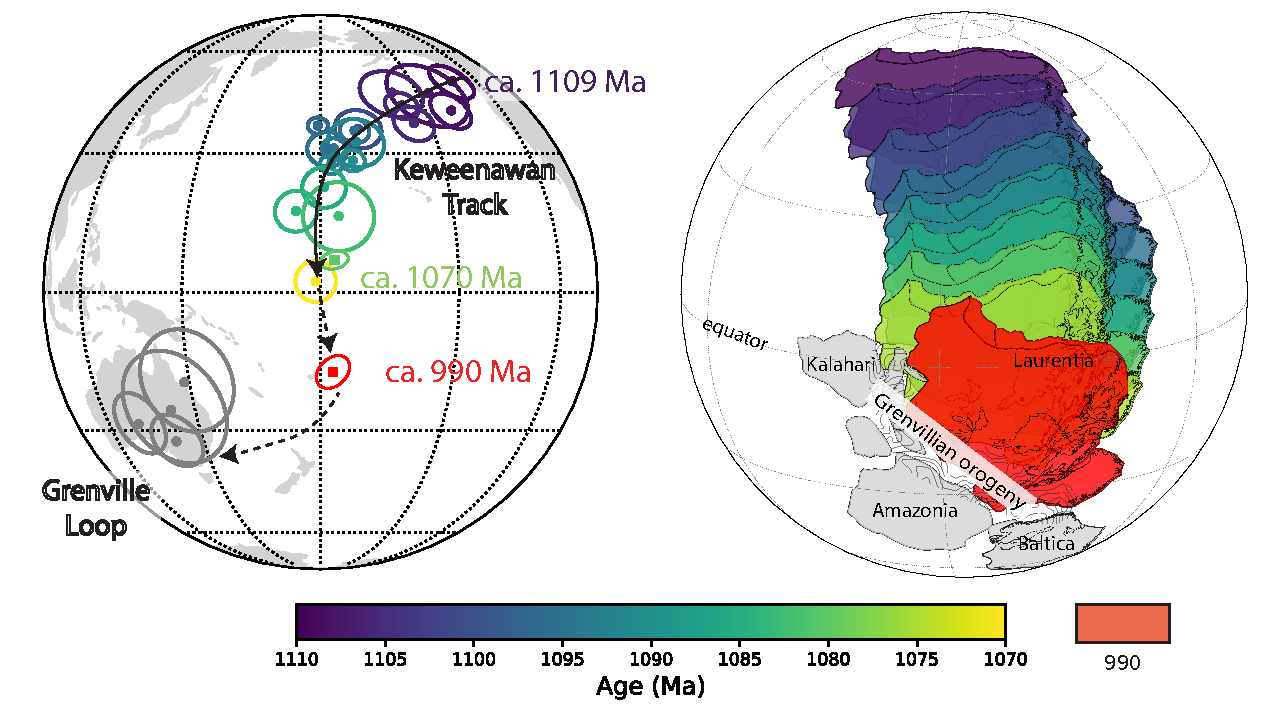
\includegraphics[width=\textwidth]{figure/pole_summary.pdf}
    \caption[Summary paleomagnetic data and paleogeography reconstruction for Laurentia through the late Mesoproterozoic to the early Neoproterozoic.]{Summary paleomagnetic data and paleogeography reconstruction for Laurentia through the late Mesoproterozoic to the early Neoproterozoic. Left panel shows a compilation of paleomagnetic poles that constructs the ca. 1109-1070 Ma Keweenawan Track, the ca. 990 Ma Jacobsville Formation pole, and representative paleomagnetic poles developed from rocks of the Grenville orogen. Right panel shows a snapshot of paleogeography reconstruction ca. 990 Ma. Positions of Laurentia and the conjugate continents along Laurentia's present-day eastern margin where the Grenvillian orogenesis occurred are reconstructed based on the Jacobsville pole and previously published paleomagnetic and geologic constraints. The details of the data compilation and reconstructions are presented in Chapter 3.}
    \label{fig:abstract_paleogeography}
\end{figure}

Rocks of the Grenville orogen experienced granulite facies metamorphism with temperatures up to 950\textdegree C \citep{Shinevar2021a, Metzger2021a} which exceeds the Curie temperature of magnetite (580\textdegree C) and N\'eel temperature of hematite (690\textdegree C). As a result, the remanent magnetization that the rocks acquired during initial formation was entirely erased by heating during peak metamorphism, and subsequently overwritten during cooling associated with exhumation \citep{McWilliams1975a}. Therefore, these rocks have the potential to provide additional insights into the global paleogeography following Grenville peak metamorphism. Previously, a large amount of paleomagnetic data have been developed from rocks of the Grenville orogen. The paleomagnetic poles cluster in a distinct position that is south to the end of the Keweenawan Track and also south to the ca. 990 Ma Jacobsville Formation pole (Fig. \ref{fig:abstract_paleogeography}). 

However, it is challenging to precisely determine the age of the Grenville poles. Determining the age of the the timing of remanence acquisition in rocks of the Grenville orogen requires constraining the cooling history of the orogen. Pioneering work that pairs thermochronology with paleomagnetic data recognized the long duration of cooling within the orogen and the necessity of determining cooling curves to assign ages to paleomagnetic poles \citep{Berger1979a}. This work has subsequently been built upon through the development of additional $^{40}$Ar/$^{39}$Ar and U-Pb thermochronology data \citep[e.g.][]{Mezger1991a, Warnock2000a} and the use of cooling curves interpreted from such data to interpret ages of paleomagnetic poles \citep[e.g.][]{Warnock2000a, Brown2012a}. As a result, high latitude Grenville Loop poles from the Haliburton intrusions in Ontario and the Adirondack Highlands have been assigned ages ranging between 1015-960 Ma. Albeit that these age assignments to Grenville Loop poles are based on rough estimates of the timing of magnetic remanence acquisition along simplified interpolation of cooling history paths with no uncertainty evaluations, they have been incorporated into curated paleomagnetic database for paleogeography reconstructions \cite[e.g.][]{Weil2003a, Evans2021a}.  

The now well-dated ca. 990 Ma configuration of Laurentia based on the paleomagnetic pole position of the Jacobsville Formation challenges previous configurations based on the Grenville poles. In chapter 4, robust field tests constrain the Jacobsville pole to be a primary detrital remanent magnetization that is chronostratigraphically well-constrained. We consider it to be a reliable representation of the position of Laurentia ca. 990 Ma. That the ages assigned to the Grenville Loop poles are both the same and bracketing the age of the Jacobsville pole presents a conundrum given the very different positions they imply for Laurentia and associated continents in Rodinia. However, it is not feasible to invoke a model where Laurentia and the Grenville Province were separated at the time of Jacobsville Formation deposition, since geochornology data show that it was deposited in a synorogenic basin as the Grenville Front developed and propagated into the interior of Laurentia during the last pulse of Grenvillian contractional deformation. Alternatively, I hypothesize that the Grenville poles must be a representation of Laurentia's paleogeographic position, but the question is at what time? 

In previous Grenville paleomagnetic literature, the lack of reporting uncertainties associated with these age assignments is partly due to the lack of using quantitative methods to reconstruct probable thermal history paths based on the available thermochronology data. The fact that measurement level data and specimen-specific details such as grain sizes are not available for the historic thermochronology literature makes it difficult to reproduce or improve those estimated ages for remanence acquisition. Additional uncertainty that was not fully taken into account in the previous literature comes from the cooling-rate dependence of magnetic remanence acquisition. In some contributions that have assigned ages to Grenville paleomagnetic poles, the Curie temperature of magnetite has been used as the temperature with which to assign an age to a magnetite magnetization from an interpreted cooling curve. While the Curie temperature is certainly relevant, as above it the mineral is paramagnetic rather than ferromagnetic, blocking temperatures for an assemblage of grains will be below the Curie temperature. For populations of pre-existing magnetite, acquisition of magnetization occurs as a rock cools through temperatures where the thermal fluctuation energy is no longer sufficient to reset the magnetization of particles to align with the ambient field on a given timescale (the relaxation time). For rapidly cooled rocks such as lava flows, the cooling rate during emplacement and that during demagnetization in the lab are similar and the observed unblocking temperatures in the lab are close to the natural blocking temperatures during remanence acquisition. In contrast to a rapidly cooled lava, magnetite-bearing rocks in the Grenville orogen acquired remanence during protracted cooling after peak metamorphism leading to a several orders of magnitude difference between the natural cooling rate and thermal demagnetization in the lab. This slow cooling leads to an expression of the cooling rate dependence where the temperatures at which a magnetization is acquired are lower than the temperatures at which it is removed in the lab \citep{Pullaiah1975b, Halgedahl1980a, Dodson1980a}. Estimating the age of remanence acquisition in conjunction with cooling trajectories necessitates developing a framework that implements these relationships. These considerations further highlight the importance of precisely determining the unblocking temperatures of magnetite-held remanence associated with a paleomagnetic direction. Previous efforts to assign ages based on cooling curves have typically picked single temperature values. 

In the future, I am interested in testing a hypothesis that the poles from the Grenville orogen are younger than currently interpreted. Instead of the poles having remanence that was acquired while the Grenvillian orogeny was still ongoing (as is the case of the interpretation of the Haliburton pole; \citealp{Warnock2000a}) or in the few tens of millions of years following the Rigolet stage, the magnetic remanence could instead have been acquired during exhumation well after the ca. 980 Ma cessation of contractional deformation. In this scenario, the migration of Rodinia to the higher latitude position represented by the Grenville Loop poles would have occurred further into the Neoproterozoic (Fig. \ref{fig:abstract_paleogeography}). Testing this hypothesis is of central importance to Neoproterozoic paleogeography as the ages associated with those Grenville Loop poles are crucial for constraining the motion of Laurentia at this time and the configuration between Laurentia and hypothesized conjugate continents. For example, in the case of Baltica it has been argued through comparison between paleomagnetic poles from the Grenville orogen and Sveconorwegian orogen that there were multiple oscillatory true polar wander rotations in the early Neoproterozoic \citep{Evans2015a, Gong2018a}. This interpretation is reliant on the assigned ages of the poles in both orogens. I plan to approach this question by developing high-precision U-Pb thermochronology data and new high-resolution paleomagnetic data. I will quantitatively construct thermal history paths and associated uncertainties using U-Pb apatite system as a thermochronometer which have closure temperatures similar to the blocking temperatures of titanomagnetite in Grenville rocks. I will pair these results with new high-resolution thermal demagnetization data such that the natural blocking temperature of the Grenville rocks can be better constrained based on the unblocking spectra obtained in the lab, taking the cooling-rate effect into consideration. 

\end{abstract}
